\section{Co-Operation: Multi-Turn --- AI Level Generation
Project}\label{co-operation-multi-turn-ai-level-generation-project}

\textbf{Client:} Shaz Yousaf --- Mind Feast Games

\textbf{Group 1}

\begin{longtable}[]{@{}ll@{}}
\toprule\noalign{}
Group Member & Role \\
\midrule\noalign{}
\endhead
\bottomrule\noalign{}
\endlastfoot
David Williams & Group Admin \& Python Automation \\
Harrison McDevitt & AI Research \& Lua \\
Oscar Kennedy & Lead Level Designer \\
Mervin Manuel & GUI Level Editor \& Secondary Group Admin \\
\end{longtable}

\begin{center}\rule{0.5\linewidth}{0.5pt}\end{center}

\section{Table of Contents}\label{table-of-contents}

\begin{enumerate}
\def\labelenumi{\arabic{enumi}.}
\tightlist
\item
  \hyperref[introduction]{Introduction}
\item
  \hyperref[project-management]{Project Management}

  \begin{itemize}
  \tightlist
  \item
    2.1 \hyperref[21-team-structure--communication]{Team Structure \&
    Communication}
  \item
    2.2 \hyperref[22-sprint-planning--timeline]{Sprint Planning \&
    Timeline}
  \item
    2.3 \hyperref[23-risk-management]{Risk Management}
  \end{itemize}
\item
  \hyperref[design]{Design}

  \begin{itemize}
  \tightlist
  \item
    3.1 \hyperref[31-initial-ai-level-generation-concept]{Initial AI
    Level Generation Concept}
  \item
    3.2 \hyperref[32-the-agentic-approach]{The Agentic Approach}
  \item
    3.3 \hyperref[33-the-pivot-from-generation-to-authoring]{The Pivot:
    From Generation to Authoring}
  \item
    3.4 \hyperref[34-level-editor-architecture]{Level Editor
    Architecture}
  \item
    3.5 \hyperref[35-development-process-with-opencode]{Development
    Process with OpenCode}
  \item
    3.6 \hyperref[36-uml-diagrams]{UML Diagrams}
  \end{itemize}
\item
  \hyperref[quality-assurance--testing]{Quality Assurance \& Testing}

  \begin{itemize}
  \tightlist
  \item
    4.1 \hyperref[41-unit-tests]{Unit Tests}
  \item
    4.2 \hyperref[42-integration--functional-tests]{Integration \&
    Functional Tests}
  \end{itemize}
\item
  \hyperref[conclusion]{Conclusion}
\item
  \hyperref[references]{References}
\item
  \hyperref[appendix-personal-reflections]{Appendix: Personal
  Reflections}
\end{enumerate}

\begin{center}\rule{0.5\linewidth}{0.5pt}\end{center}

\section{Introduction}\label{introduction}

\begin{figure}
\centering
\pandocbounded{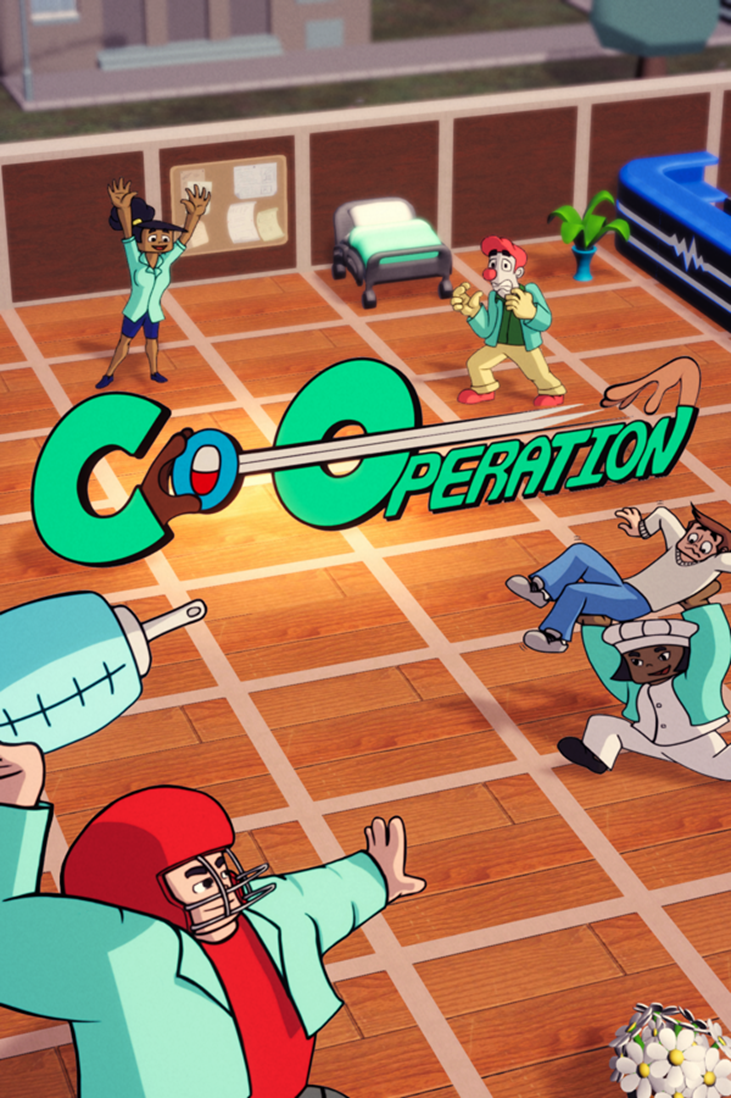
\includegraphics[keepaspectratio]{images/co-operation title.png}}
\caption{Cover art for the game.}
\end{figure}

Co-Operation: Multi-Turn is a game created by Mind Feast Games (founded
in 2020) that is centred around a turn-based gameplay loop of healing
and relocating patients within a comedic hospital setting and getting
them the correct medicine in a timely manner. Mind Feast Games create
games as part of an initiative to encourage people to collaborate and
connect with one another --- something the studio achieved convincingly
with this title. A standout aspect of the game is the integration of
mobile devices to control the on-screen characters, implemented in a
similar vein to the Jackbox series. Players queue up a set of actions
that play out on a shared screen, and the ability to join a lobby from
any browser-capable device --- phone, laptop, tablet --- makes the
experience uniquely portable. Movement must be coordinated actively for
the game to run smoothly, and the lively group discussion this demands
regularly produces comical moments when a wrong move is chosen.

\begin{figure}
\centering
\pandocbounded{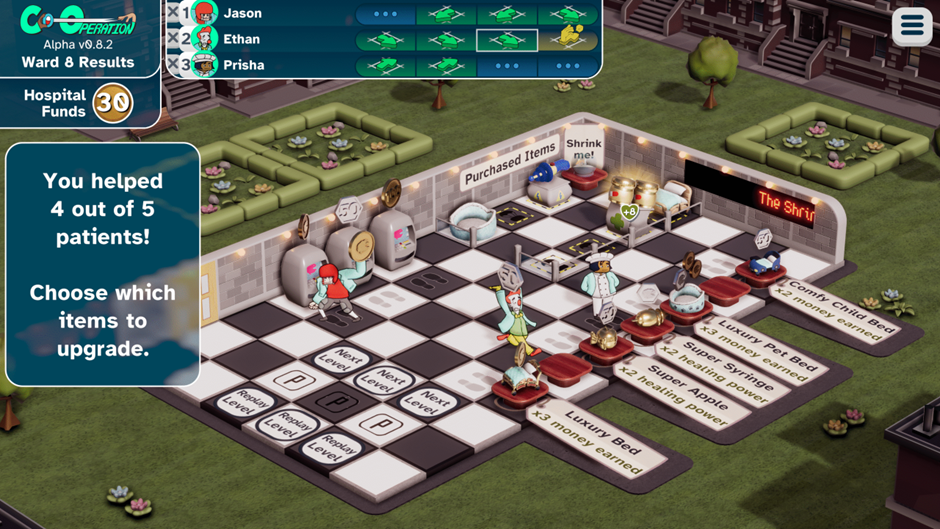
\includegraphics[keepaspectratio]{images/level preview intro.png}}
\caption{Initial preview of game.}
\end{figure}

We played the game as a group to gauge its gameplay loop and understand
how the levels were structured. We found a lot of heart in the design,
and the level layouts complemented the core game loop well across all of
the base-game content. We had fun dissecting the various traversal
avenues available to the player and examining how each prop altered
movement possibilities differently --- for example, low barriers allow
items and patients to be thrown over them, while solid walls block
movement entirely. During this play session we began forming early ideas
about how we might approach level generation.

\begin{figure}
\centering
\pandocbounded{
\includegraphics[keepaspectratio]{images/drawn players playing game.png}}
\caption{Initial preview of game.}
\end{figure}

The brief from our client, Mind Feast Games, asked us to create AI tools
capable of generating an arbitrary number of levels that were cohesive,
fun to play, and of comparable quality to the base game's existing
content. The intended workflow was for levels to be generated externally
and hand-picked by the developers before being included in a future
release. This placed a premium on quality over quantity: generated
levels needed to be architecturally sound and capable of sitting
alongside professionally designed content without feeling out of place.

Understanding the level file format was the essential first step. Levels
in Co-Operation: Multi-Turn are defined entirely in YAML files. A level
consists of a two-dimensional grid of two-character alphanumeric tile
codes, a \texttt{gridObjects} section that maps each code to an ordered
list of game objects, a \texttt{cameraSettings} block, and an
\texttt{include} directive that pulls in shared asset definitions from a
file called \texttt{LevelsShared.yaml}. A tile such as \texttt{f}
denotes a floor tile, \texttt{2b} a particular building variant, and the
special code \texttt{gm} anchors the level's management and scoring
systems. This structure is both expressive and precise --- even a small
formatting error in the YAML causes the game engine to refuse to load
the level.

\begin{quote}
\textbf{Game Format Summary:} Levels are defined as YAML files
containing: an \texttt{include} directive pointing to
\texttt{LevelsShared.yaml}; a \texttt{sceneName} indicating the Unity
background scene; a \texttt{grid} block storing comma-separated
2-character tile codes as a literal block scalar (\texttt{\textbar{}});
a \texttt{gridObjects} section mapping each code to an ordered list of
objects; \texttt{cameraSettings}; and an \texttt{objectDefinitions}
section for user-defined tile presets.
\end{quote}

\begin{center}\rule{0.5\linewidth}{0.5pt}\end{center}

\section{Project Management}\label{project-management}

\subsection{2.1 Team Structure \&
Communication}\label{team-structure-communication}

The team was composed of four members with complementary skillsets.
\textbf{David Williams} assumed the role of Group Admin, coordinating
task allocation, maintaining the shared repository, and leading the
Python automation work. \textbf{Harrison McDevitt} was responsible for
AI research and explored Lua scripting as a potential route for
in-engine level validation. \textbf{Oscar Kennedy}, as Lead Level
Designer, contributed domain expertise and designed the six hand-crafted
levels that formed part of the final deliverable. \textbf{Mervin Manuel}
took responsibility for the GUI Level Editor and served as Secondary
Group Admin.

Communication was maintained through a shared messaging channel and
regular in-person meetings during university contact hours. Version
control was handled via Git, with each team member working on feature
branches before merging to a shared main branch. Code reviews were
conducted informally but consistently throughout Semester 2.

\begin{longtable}[]{@{}
  >{\raggedright\arraybackslash}p{(\linewidth - 2\tabcolsep) * \real{0.5000}}
  >{\raggedright\arraybackslash}p{(\linewidth - 2\tabcolsep) * \real{0.5000}}@{}}
\toprule\noalign{}
\begin{minipage}[b]{\linewidth}\raggedright
Member
\end{minipage} & \begin{minipage}[b]{\linewidth}\raggedright
Primary Responsibilities
\end{minipage} \\
\midrule\noalign{}
\endhead
\bottomrule\noalign{}
\endlastfoot
David Williams & Project coordination, Python scripting, YAML automation
pipeline, documentation \\
Harrison McDevitt & AI research (LLM prompt engineering, agentic testing
concept), Lua scripting, QA planning \\
Oscar Kennedy & Level design philosophy, six hand-crafted levels,
playability review \\
Mervin Manuel & GUI level editor (Python/Tkinter), YAML integration, UX
iteration, secondary admin \\
\end{longtable}

\subsection{2.2 Sprint Planning \&
Timeline}\label{sprint-planning-timeline}

The project spanned two semesters. Semester 1 was largely exploratory
--- the team spent considerable time understanding the game's data
format, playing existing levels, and researching generative approaches.
This period was valuable for building domain knowledge but produced no
concrete technical output, and it created a dependency on strategic
decisions that were deferred into Semester 2.

Semester 2 was divided into informal two-week sprints. The first sprint
was dedicated entirely to resolving the overarching strategic question:
what would the team actually build? The subsequent sprints tracked the
following milestones:

\begin{itemize}
\tightlist
\item
  \textbf{Sprint 1 (Weeks 1--2):} Strategic decision confirmed --- pivot
  to GUI editor; YAML format research completed.
\item
  \textbf{Sprint 2 (Weeks 3--4):} Core Tkinter grid editor prototype;
  YAML load/save working end-to-end.
\item
  \textbf{Sprint 3 (Weeks 5--6):} Visual tile rendering via GLB texture
  extraction; mod folder integration.
\item
  \textbf{Sprint 4 (Weeks 7--8):} Paint tool, camera settings editor,
  Ctrl+S saving, close-prompt for unsaved changes.
\item
  \textbf{Sprint 5 (Weeks 9--10):} Undo/redo stack, quick palette
  dropdown, user-defined grid codes.
\item
  \textbf{Sprint 6 (Weeks 11--12):} Final polish, comment pass through
  all code, README update, level hand-off to Oscar.
\end{itemize}

\subsection{2.3 Risk Management}\label{risk-management}

Several risks were identified throughout the project, some of which
materialised and required active mitigation.

The most significant risk was \textbf{scope ambiguity}. The original
brief called for AI level generation, but no single approach was agreed
upon during Semester 1. This led to the primary challenge described in
Section 3 --- prolonged indecision about which generation strategy to
pursue. The team mitigated this by formally deciding at the start of
Semester 2 to produce a high-quality tool rather than a
partially-working generative algorithm.

A secondary risk was \textbf{technical compatibility with the game's
YAML dialect}. The game uses custom YAML tags such as
\texttt{!SpineAnimation} and \texttt{!MeshDeformAnimation} ---
non-standard constructs that Python's default \texttt{yaml.safe\_load}
rejects with a \texttt{ConstructorError}. Mervin addressed this by
writing custom tag constructors for each known type, plus a generic
multi-constructor fallback for any unknown tags encountered at runtime.

A third risk was \textbf{asset integration for tile visualisation}. The
editor needed to display tile textures, but the game's textures were
embedded inside GLB (binary GLTF) 3D model files rather than standalone
image assets. This required implementing texture extraction via the
\texttt{pygltflib} library, with a fallback to coloured rectangles when
extraction was not possible.

\begin{quote}
\textbf{Key Risk Summary:} The three main risks were: (1) strategic
indecision leading to project delays --- mitigated by a formal scope
pivot; (2) YAML parsing failures due to custom tags --- mitigated by
custom constructors; (3) missing tile textures --- mitigated by GLB
texture extraction with colour fallback.
\end{quote}

\begin{center}\rule{0.5\linewidth}{0.5pt}\end{center}

\section{Design}\label{design}

\subsection{3.1 Initial AI Level Generation
Concept}\label{initial-ai-level-generation-concept}

The project's original intention was fully automated level generation.
Early team discussions centred on procedural content generation (PCG)
techniques that could produce valid YAML level files without human
authorship. Three broad approaches were explored during Semester 1.

\subsubsection{Constraint-Based
Generation}\label{constraint-based-generation}

The first approach involved using a constraint solver or search
algorithm to explore the space of valid level configurations. Given the
game's grid format and the set of known tile codes, such a system could
theoretically enumerate layouts satisfying a set of design rules ---
minimum floor coverage, at least one patient and one medicine cabinet, a
reachable path between all key objects. The fundamental challenge was
defining what ``valid'' meant beyond technical well-formedness. A grid
that loads without errors is not the same as a grid that constitutes a
fun, balanced level. Encoding playability as constraints proved more
complex than initially anticipated.

\subsubsection{Example-Based Generation}\label{example-based-generation}

The second approach used the existing base-game levels as a training
corpus. A generative model could learn patterns of tile placement and
produce novel arrangements that preserved those statistical regularities
--- analogous to texture synthesis or Markov-chain map generation. A
prototype was briefly sketched using bigram tile transition
probabilities. However, the base game contained too few levels for
meaningful pattern extraction, and the resulting outputs lacked the
intentionality of hand-crafted design.

\subsubsection{LLM-Driven Generation}\label{llm-driven-generation}

The third and most ambitious approach drew on large language models.
Harrison investigated whether a language model --- provided with the
game's YAML format documentation and example levels --- could generate
new levels as structured text outputs. Initial experiments were
promising in that the model understood the format and produced
syntactically valid YAML. However, semantic coherence was inconsistent:
the model would sometimes place patient spawn points without
corresponding medicine cabinets, define grid codes in the \texttt{grid}
block that had no entry in \texttt{gridObjects}, or produce layouts with
unreachable areas. Validating and correcting this output would itself
require detailed game-engine knowledge that the team did not have access
to at runtime.

\begin{quote}
\textbf{LLM Generation Challenges:} When prompted to generate level
YAML, language models produced structurally valid output but frequently
introduced semantic errors --- missing \texttt{objectDefinitions}
entries for referenced codes, incorrect \texttt{include} directive
syntax, and layout configurations that produced unreachable game areas.
Correcting these errors required game-engine knowledge that could not be
automated without a runtime validator.
\end{quote}

\subsection{3.2 The Agentic Approach}\label{the-agentic-approach}

One of the most intellectually stimulating avenues explored by the team
was an agentic AI approach to level testing and validation. The concept,
developed by Harrison, was inspired by emerging work in AI game testing:
rather than having a human play a generated level to check for problems,
an AI agent could be given a description of the game's rules and tasked
with playing the level autonomously, logging any issues it encountered.

The envisioned architecture was a feedback loop: an LLM-based agent
would receive the current level's YAML, a description of the game
mechanics, and access to a set of ``test actions'' it could perform ---
checking whether every patient had a corresponding medicine cabinet,
whether all floor tiles were reachable from the spawn point, whether the
game management objects were correctly placed at the \texttt{gm} tile.
The agent would produce a structured bug report, which could either be
fed back to a generative model for correction or surfaced to a human
level designer for review.

This approach was appealing because it separated the concerns of
generation and validation. A generative model need not produce perfect
output on the first pass; instead, it could produce a rough layout that
an agentic tester would critique, and the cycle would iterate toward a
playable level over successive rounds.

However, the approach encountered a fundamental practical obstacle.
\textbf{The game engine is a closed Unity binary --- there was no
exposed API through which an agent could programmatically query the game
state or run a level headlessly.} The team had no access to the game's
source code and could not instrument it for automated testing. Without
the ability to run levels in a controllable environment, the agentic
tester was reduced to static analysis of the YAML file --- useful, but a
significant reduction from the full runtime validation the concept had
promised.

Static YAML analysis was implemented in a limited form as part of
David's Python automation scripts. These scripts checked for: orphaned
GridObject references (codes that appeared in \texttt{grid} but had no
corresponding \texttt{gridObjects} entry), missing
\texttt{objectDefinitions} entries, and invalid grid dimensions. These
checks caught common structural errors but could not detect emergent
gameplay problems such as level imbalance, inaccessible areas, or unfair
patient-to-medicine distances, which only manifest at runtime.

\subsection{3.3 The Pivot: From Generation to
Authoring}\label{the-pivot-from-generation-to-authoring}

By the midpoint of Semester 2 it became clear that fully automated AI
level generation was not achievable within the remaining timeframe. Each
of the three generative approaches had fundamental blockers that could
not be resolved quickly, and the agentic testing concept --- while
architecturally sound --- was stymied by the game engine's opacity.

This realisation prompted a period of honest reflection. The team had
invested considerable time in research and had little shipped tooling to
show for it. The risk of submitting a partially-working generative
algorithm --- one that produced technically valid YAML but levels of
questionable quality --- was weighed against pivoting to a different
deliverable entirely.

The pivot decision was made collectively. Rather than abandoning the
project's AI dimension, the team reframed the problem: \textbf{a
high-quality GUI level editor, designed with deep awareness of the
game's format, would become the primary deliverable.} This reframing
served two purposes simultaneously. First, the editor would directly
accelerate human-authored level creation, allowing the client's team to
produce expansion content without manual YAML editing. Second, the
levels created with it --- along with the editor's documented format
rules --- would constitute a structured training corpus for a future AI
pipeline. The \texttt{skills.md} file produced alongside the editor was
explicitly designed with this future use case in mind.

This pivot was informed by pragmatic constraints, but it also carried
genuine value. The resulting editor is a sophisticated tool that
non-technical designers can use productively, and it delivers on the
core promise of the brief --- making it faster and easier to create more
levels for Co-Operation: Multi-Turn.

\begin{quote}
\textbf{Pivot Rationale:} The pivot was driven by three factors: (1)
insufficient training data for example-based models; (2) lack of runtime
API access for agentic testing; (3) LLM output requiring domain-expert
validation that was itself more expensive than manual design. The editor
reframes AI-assistance as future-compatible infrastructure rather than
an immediate deliverable.
\end{quote}

\subsection{3.4 Level Editor
Architecture}\label{level-editor-architecture}

The level editor, \texttt{level\_editor.py}, is a single-file Python
application built on the Tkinter GUI framework. It follows an RPG
Maker-inspired dual-panel design --- separating tile grid editing (the
map layer) from GridObject editing (the event/object layer). This
mirrors the conceptual distinction the game engine itself draws between
the \texttt{grid} (which defines spatial layout) and the
\texttt{gridObjects} section (which attaches behaviour and entities to
each cell).

\subsubsection{Core Data Model}\label{core-data-model}

The application maintains two primary data structures: a two-dimensional
list (\texttt{grid\_data}) storing the two-character code occupying each
cell, and a dictionary (\texttt{grid\_objects}) mapping each code to its
ordered list of GridObject definitions. These are kept in sync
throughout the session and serialised to YAML on save.

\subsubsection{YAML Handling}\label{yaml-handling}

One of the editor's most technically demanding components is its YAML
subsystem. The game uses a superset of YAML that includes custom tags
such as \texttt{!SpineAnimation}, \texttt{!GLBAnimation},
\texttt{!TweenAnimation}, and \texttt{!MeshDeformAnimation}. Python's
PyYAML library rejects these by default with a
\texttt{ConstructorError}. The editor addresses this with a suite of
custom constructors registered at module load time:

\begin{Shaded}
\begin{Highlighting}[]
\KeywordTok{class}\NormalTok{ TaggedObject(}\BuiltInTok{dict}\NormalTok{):}
    \CommentTok{"""Dict subclass that remembers its YAML tag for round{-}trip serialisation."""}
    \KeywordTok{def} \FunctionTok{\_\_init\_\_}\NormalTok{(}\VariableTok{self}\NormalTok{, }\OperatorTok{*}\NormalTok{args, }\OperatorTok{**}\NormalTok{kwargs):}
\NormalTok{        tag }\OperatorTok{=}\NormalTok{ kwargs.pop(}\StringTok{\textquotesingle{}\_tag\textquotesingle{}}\NormalTok{, }\VariableTok{None}\NormalTok{)}
        \BuiltInTok{super}\NormalTok{().}\FunctionTok{\_\_init\_\_}\NormalTok{(}\OperatorTok{*}\NormalTok{args, }\OperatorTok{**}\NormalTok{kwargs)}
        \VariableTok{self}\NormalTok{.\_tag }\OperatorTok{=}\NormalTok{ tag}

\KeywordTok{def}\NormalTok{ tagged\_object\_representer(dumper, data):}
\NormalTok{    tag }\OperatorTok{=} \BuiltInTok{getattr}\NormalTok{(data, }\StringTok{\textquotesingle{}\_tag\textquotesingle{}}\NormalTok{, }\VariableTok{None}\NormalTok{)}
    \ControlFlowTok{if}\NormalTok{ tag:}
        \ControlFlowTok{return}\NormalTok{ dumper.represent\_mapping(}\SpecialStringTok{f\textquotesingle{}!}\SpecialCharTok{\{}\NormalTok{tag}\SpecialCharTok{\}}\SpecialStringTok{\textquotesingle{}}\NormalTok{, }\BuiltInTok{dict}\NormalTok{(data))}
    \ControlFlowTok{return}\NormalTok{ dumper.represent\_mapping(}\StringTok{\textquotesingle{}tag:yaml.org,2002:map\textquotesingle{}}\NormalTok{, }\BuiltInTok{dict}\NormalTok{(data))}

\NormalTok{yaml.add\_representer(TaggedObject, tagged\_object\_representer)}
\end{Highlighting}
\end{Shaded}

A \texttt{TaggedObject} is a dictionary subclass that remembers the YAML
tag that produced it, allowing complete round-trip serialisation without
data loss. Alongside the named constructors, a generic multi-constructor
handles any unknown custom tag the editor encounters in the wild:

\begin{Shaded}
\begin{Highlighting}[]
\KeywordTok{def}\NormalTok{ generic\_tag\_handler(loader, suffix, node):}
    \ControlFlowTok{if} \BuiltInTok{isinstance}\NormalTok{(node, yaml.MappingNode):}
\NormalTok{        data }\OperatorTok{=}\NormalTok{ loader.construct\_mapping(node)}
        \ControlFlowTok{return}\NormalTok{ TaggedObject(data, \_tag}\OperatorTok{=}\NormalTok{suffix)}
    \ControlFlowTok{elif} \BuiltInTok{isinstance}\NormalTok{(node, yaml.SequenceNode):}
\NormalTok{        data }\OperatorTok{=}\NormalTok{ loader.construct\_sequence(node)}
        \ControlFlowTok{return}\NormalTok{ TaggedObject(\{}\StringTok{\textquotesingle{}\_data\textquotesingle{}}\NormalTok{: data, }\StringTok{\textquotesingle{}\_tag\textquotesingle{}}\NormalTok{: suffix\})}
    \ControlFlowTok{else}\NormalTok{:}
\NormalTok{        data }\OperatorTok{=}\NormalTok{ loader.construct\_scalar(node)}
        \ControlFlowTok{return}\NormalTok{ TaggedObject(\{}\StringTok{\textquotesingle{}\_value\textquotesingle{}}\NormalTok{: data, }\StringTok{\textquotesingle{}\_tag\textquotesingle{}}\NormalTok{: suffix\})}

\NormalTok{yaml.add\_multi\_constructor(}\StringTok{\textquotesingle{}!\textquotesingle{}}\NormalTok{, generic\_tag\_handler, Loader}\OperatorTok{=}\NormalTok{yaml.SafeLoader)}
\end{Highlighting}
\end{Shaded}

The editor also implements full \textbf{YAML include resolution}. When a
level file contains an \texttt{include} directive (typically pointing to
\texttt{LevelsShared.yaml}), the editor recursively loads the referenced
file and merges its contents into the working data model. Circular
includes are detected via a set of already-visited absolute paths and
reported as warnings. The original include list is preserved in the
serialised output so saved files retain the correct \texttt{include}
directive rather than inlining all shared definitions.

\subsubsection{Visual Tile Rendering}\label{visual-tile-rendering}

The game's tile assets are stored as 3D GLB models rather than 2D
sprites, which created an unexpected challenge. The editor's first
rendering strategy attempted to locate PNG files in the game's
\texttt{art/2d} folder, matching filenames to the tile codes defined in
\texttt{LevelsShared.yaml}. This worked for a subset of tiles but failed
for the majority, which had no standalone 2D asset.

The fallback strategy uses the \texttt{pygltflib} library to open each
tile's GLB file and extract its albedo texture. GLB files can contain
multiple material textures; the editor specifically targets the albedo
(base colour) map rather than normal or specular maps. Extracted
textures are cached as PIL \texttt{Image} objects and resized to cell
dimensions for display. When no texture can be extracted, cells fall
back to a distinctive coloured rectangle derived from the tile code's
hash.

\subsubsection{User Interaction
Features}\label{user-interaction-features}

The editor's feature set was informed directly by a detailed development
conversation with the client, iterating through OpenCode. Key features
include:

\begin{itemize}
\tightlist
\item
  \textbf{RPG Maker-style paint tool:} right-click and drag to paint the
  current tile code across multiple cells.
\item
  \textbf{Ctrl+Right-click eraser:} clears painted cells without
  changing the current selection.
\item
  \textbf{Scroll-wheel zoom:} smoothly scales the grid view between
  configurable minimum and maximum zoom levels.
\item
  \textbf{Middle-click pan:} repositions the viewport over large grids
  without the scrollbars.
\item
  \textbf{Undo/Redo (Ctrl+Z / Ctrl+Shift+Z):} a capped history stack of
  50 grid states enables non-destructive experimentation.
\item
  \textbf{Quick palette:} a dropdown populated from both the game's
  shared definitions and user-defined grid codes.
\item
  \textbf{Camera settings editor:} a pop-up dialog for all
  \texttt{cameraSettings} fields with per-field reset-to-default
  buttons.
\item
  \textbf{Ctrl+S save:} serialises the current level to YAML with a
  close-prompt safeguard for unsaved changes.
\end{itemize}

\subsection{3.5 Development Process with
OpenCode}\label{development-process-with-opencode}

The level editor was developed using OpenCode, an AI-assisted coding
tool, in a conversational and iterative fashion. The development
conversation --- preserved in the project's documentation --- reveals a
pattern characteristic of this kind of AI-assisted development: the
developer poses a high-level requirement, the AI produces an
implementation, the developer tests it, identifies problems, and feeds
those problems back as subsequent prompts.

The initial request was deliberately broad: \emph{given documentation of
the YAML format and an example level file, build a Python Tkinter editor
focused on grid editing with separate GridObject creation, similar to
RPG Maker.} The AI produced a functional prototype in a single response,
but iteration was required immediately: the YAML include system was
broken, the mod folder structure was not correctly inferred, and there
was no visual tile rendering.

Each of these issues became its own conversation thread. The include
directive support was addressed first, then folder inference, then
texture rendering. Texture rendering required three successive
refinements before working correctly: the initial implementation
attempted to load PNG files directly, then switched to GLB extraction
but loaded normal maps instead of albedo maps, and finally correctly
targeted albedo textures after the developer inspected the temp folder
and reported the symptom.

This process demonstrated both the power and the practical limits of
AI-assisted coding. The AI produced large, structurally sound code
blocks rapidly, but it required precise, symptom-level feedback to
converge on correct behaviour. Features like undo/redo, the paint tool,
and the quick palette were added incrementally without breaking existing
functionality, reflecting the quality of the underlying architecture the
AI had established.

A particularly instructive episode concerned reducing YAML output file
size. Early versions of the editor copied the entire contents of
\texttt{LevelsShared.yaml} into each saved level file. This produced
multi-thousand-line documents that failed to load in the game engine
with the error:

\begin{verbatim}
Value for parameter 'objectDefinitions' not found in deserialized data
for type 'cooperation.model.levels.CoOperationLevelDefinition'
\end{verbatim}

The fix required understanding the game engine's precise expectations:
\texttt{objectDefinitions:\ \{\}} must be present even when empty, and
the level file must contain an
\texttt{include:\ {[}LevelsShared.yaml{]}} directive rather than
inlining the shared content. Restructuring the save logic to emit only
the minimal required keys resolved the issue.

\subsection{3.6 UML Diagrams}\label{uml-diagrams}

\subsubsection{Class Overview}\label{class-overview}

The editor's architecture is organised around three primary
responsibilities: data management, rendering, and user interaction. The
five main classes are described below.

\textbf{\texttt{LevelEditorApp}} is the root class, inheriting from
\texttt{tk.Tk}. It owns the central data structures: \texttt{grid\_data}
(2D list of tile codes), \texttt{grid\_objects} (dict mapping codes to
GridObject lists), \texttt{object\_definitions} (dict of user-defined
tile presets), and the undo/redo stacks. It manages the overall layout
--- menu bar, scrollable canvas grid panel, side palette panel --- and
dispatches all keyboard shortcuts.

\begin{Shaded}
\begin{Highlighting}[]
\NormalTok{@startuml LevelEditor Class Diagram}
\NormalTok{class LevelEditor \{}
\NormalTok{    {-} root : Tk}
\NormalTok{    {-} grid\_data : list}
\NormalTok{    {-} grid\_objects : dict}
\NormalTok{    {-} object\_definitions : dict}
\NormalTok{    {-} current\_file : str}
\NormalTok{    {-} streaming\_assets\_path : str}
\NormalTok{    {-} available\_assets : dict}
\NormalTok{    {-} shared\_defs\_path : StringVar}
\NormalTok{    {-} shared\_data : dict}
\NormalTok{    {-} full\_yaml\_data : dict}
\NormalTok{    {-} loaded\_includes : list}
\NormalTok{    + \_\_init\_\_(root : Tk)}
\NormalTok{\}}
\NormalTok{@enduml}
\end{Highlighting}
\end{Shaded}

\begin{Shaded}
\begin{Highlighting}[]
\KeywordTok{class}\NormalTok{ LevelEditor:}
    \CommentTok{"""Main Level Editor application"""}
    \KeywordTok{def} \FunctionTok{\_\_init\_\_}\NormalTok{(}\VariableTok{self}\NormalTok{, root):}
        \VariableTok{self}\NormalTok{.root }\OperatorTok{=}\NormalTok{ root}
        \VariableTok{self}\NormalTok{.root.title(}\StringTok{"Co OPERATION: MultiTurn {-} Level Editor"}\NormalTok{)}
        \VariableTok{self}\NormalTok{.root.geometry(}\StringTok{"1300x850"}\NormalTok{)}
        
        \CommentTok{\# Data}
        \VariableTok{self}\NormalTok{.grid\_data }\OperatorTok{=}\NormalTok{ []  }\CommentTok{\# 2D list of cell codes}
        \VariableTok{self}\NormalTok{.grid\_objects }\OperatorTok{=}\NormalTok{ \{\}  }\CommentTok{\# code {-}\textgreater{} list of objects}
        \VariableTok{self}\NormalTok{.object\_definitions }\OperatorTok{=}\NormalTok{ \{\}  }\CommentTok{\# code {-}\textgreater{} definition}
        \VariableTok{self}\NormalTok{.current\_file }\OperatorTok{=} \VariableTok{None}
        \VariableTok{self}\NormalTok{.streaming\_assets\_path }\OperatorTok{=} \VariableTok{None}
        \VariableTok{self}\NormalTok{.available\_assets }\OperatorTok{=}\NormalTok{ \{}\StringTok{\textquotesingle{}3d\textquotesingle{}}\NormalTok{: [], }\StringTok{\textquotesingle{}2d\textquotesingle{}}\NormalTok{: [], }\StringTok{\textquotesingle{}sounds\textquotesingle{}}\NormalTok{: []\}}
        
        \CommentTok{\# Shared definitions file path}
        \VariableTok{self}\NormalTok{.shared\_defs\_path }\OperatorTok{=}\NormalTok{ tk.StringVar()  }\CommentTok{\# Path to shared YAML file}
        \VariableTok{self}\NormalTok{.shared\_data }\OperatorTok{=}\NormalTok{ \{\}  }\CommentTok{\# Cached shared definitions data}
        
        \CommentTok{\# Full YAML data preservation}
        \VariableTok{self}\NormalTok{.full\_yaml\_data }\OperatorTok{=}\NormalTok{ \{\}  }\CommentTok{\# Store full YAML to preserve all sections}
        \VariableTok{self}\NormalTok{.loaded\_includes }\OperatorTok{=}\NormalTok{ []  }\CommentTok{\# Track loaded include files}
        
        \CommentTok{\# Grid state}
        \VariableTok{self}\NormalTok{.grid\_rows }\OperatorTok{=} \DecValTok{15}
        \VariableTok{self}\NormalTok{.grid\_cols }\OperatorTok{=} \DecValTok{12}
        \VariableTok{self}\NormalTok{.cell\_size }\OperatorTok{=} \DecValTok{42}
        \VariableTok{self}\NormalTok{.selected\_cell }\OperatorTok{=} \VariableTok{None}
        
        \CommentTok{\# Image display support}
        \VariableTok{self}\NormalTok{.cell\_images }\OperatorTok{=}\NormalTok{ \{\}  }\CommentTok{\# (row, col) {-}\textgreater{} canvas image id}
        \VariableTok{self}\NormalTok{.image\_cache }\OperatorTok{=}\NormalTok{ \{\}  }\CommentTok{\# (filepath, size) {-}\textgreater{} PhotoImage}
        \VariableTok{self}\NormalTok{.\_image\_refs }\OperatorTok{=}\NormalTok{ []  }\CommentTok{\# Prevent garbage collection}
        \VariableTok{self}\NormalTok{.extracted\_textures }\OperatorTok{=}\NormalTok{ \{\}  }\CommentTok{\# glb\_path {-}\textgreater{} extracted\_png\_path}
        
        \CommentTok{\# Pan state for middle{-}click panning}
        \VariableTok{self}\NormalTok{.pan\_start }\OperatorTok{=} \VariableTok{None}  \CommentTok{\# (x, y) canvas coordinates}
        
        \CommentTok{\# Selection highlight}
        \VariableTok{self}\NormalTok{.selection\_id }\OperatorTok{=} \VariableTok{None}  \CommentTok{\# Canvas item id for selection rectangle}
        
        \CommentTok{\# Painting state (RPG Maker{-}style)}
        \VariableTok{self}\NormalTok{.paint\_code }\OperatorTok{=} \VariableTok{None}  \CommentTok{\# Last applied grid code for painting}
        \VariableTok{self}\NormalTok{.painting }\OperatorTok{=} \VariableTok{False}  \CommentTok{\# Whether right{-}click painting is active}
        \VariableTok{self}\NormalTok{.erasing }\OperatorTok{=} \VariableTok{False}  \CommentTok{\# Whether Ctrl+Right{-}click eraser mode is active}
        
        \CommentTok{\# Undo/Redo system}
        \VariableTok{self}\NormalTok{.undo\_stack }\OperatorTok{=}\NormalTok{ []  }\CommentTok{\# History of previous states}
        \VariableTok{self}\NormalTok{.redo\_stack }\OperatorTok{=}\NormalTok{ []  }\CommentTok{\# States that were undone}
        \VariableTok{self}\NormalTok{.max\_undo\_history }\OperatorTok{=} \DecValTok{50}  \CommentTok{\# Maximum undo history size}
        
        \CommentTok{\# Camera settings (from YAML cameraSettings)}
        \VariableTok{self}\NormalTok{.camera\_settings }\OperatorTok{=}\NormalTok{ \{\}  }\CommentTok{\# Stores cameraSettings dict}
        
        \CommentTok{\# Setup UI}
        \VariableTok{self}\NormalTok{.setup\_menu()}
        \VariableTok{self}\NormalTok{.setup\_ui()}
        \VariableTok{self}\NormalTok{.setup\_grid()}
        
        \CommentTok{\# Initialize with empty grid}
        \VariableTok{self}\NormalTok{.init\_empty\_grid()}
        
        \CommentTok{\# Auto{-}detect Mod folder (contains Art/ and Levels/)}
        \VariableTok{self}\NormalTok{.root.after(}\DecValTok{100}\NormalTok{, }\VariableTok{self}\NormalTok{.auto\_detect\_mod\_folder)}
        
        \CommentTok{\# Bind Ctrl+S to save}
        \VariableTok{self}\NormalTok{.root.bind(}\StringTok{\textquotesingle{}\textless{}Control{-}s\textgreater{}\textquotesingle{}}\NormalTok{, }\KeywordTok{lambda}\NormalTok{ e: }\VariableTok{self}\NormalTok{.save\_yaml())}
        \VariableTok{self}\NormalTok{.root.bind(}\StringTok{\textquotesingle{}\textless{}Control{-}S\textgreater{}\textquotesingle{}}\NormalTok{, }\KeywordTok{lambda}\NormalTok{ e: }\VariableTok{self}\NormalTok{.save\_yaml())}
        
        \CommentTok{\# Bind Ctrl+Z (Undo) and Ctrl+Shift+Z (Redo)}
        \VariableTok{self}\NormalTok{.root.bind\_all(}\StringTok{\textquotesingle{}\textless{}Control{-}z\textgreater{}\textquotesingle{}}\NormalTok{, }\VariableTok{self}\NormalTok{.undo)}
        \VariableTok{self}\NormalTok{.root.bind\_all(}\StringTok{\textquotesingle{}\textless{}Control{-}Shift{-}Z\textgreater{}\textquotesingle{}}\NormalTok{, }\VariableTok{self}\NormalTok{.redo)}
        
        \CommentTok{\# Prompt on close}
        \VariableTok{self}\NormalTok{.root.protocol(}\StringTok{"WM\_DELETE\_WINDOW"}\NormalTok{, }\VariableTok{self}\NormalTok{.on\_closing)}
\end{Highlighting}
\end{Shaded}

\textbf{\texttt{GridObjectDialog}} is a modal \texttt{tk.Toplevel}
presenting a scrollable listbox of the GridObjects assigned to a
selected cell. It supports adding string-reference objects, adding
inline dictionary definitions via YAML parsing, editing existing
entries, reordering via up/down buttons, and removing entries.

\begin{Shaded}
\begin{Highlighting}[]
\KeywordTok{class}\NormalTok{ GridObjectDialog:}
    \CommentTok{"""Dialog for editing GridObjects for a single cell (like RPG Maker event editor)"""}
    \KeywordTok{def} \FunctionTok{\_\_init\_\_}\NormalTok{(}\VariableTok{self}\NormalTok{, parent, cell\_code, grid\_objects, object\_definitions, game\_assets\_path}\OperatorTok{=}\VariableTok{None}\NormalTok{):}
        \VariableTok{self}\NormalTok{.parent }\OperatorTok{=}\NormalTok{ parent}
        \VariableTok{self}\NormalTok{.cell\_code }\OperatorTok{=}\NormalTok{ cell\_code}
        \VariableTok{self}\NormalTok{.grid\_objects }\OperatorTok{=}\NormalTok{ grid\_objects}
        \VariableTok{self}\NormalTok{.object\_definitions }\OperatorTok{=}\NormalTok{ object\_definitions}
        \VariableTok{self}\NormalTok{.game\_assets\_path }\OperatorTok{=}\NormalTok{ game\_assets\_path}
        \VariableTok{self}\NormalTok{.result }\OperatorTok{=} \VariableTok{None}
        
        \VariableTok{self}\NormalTok{.dialog }\OperatorTok{=}\NormalTok{ tk.Toplevel(parent)}
        \VariableTok{self}\NormalTok{.dialog.title(}\SpecialStringTok{f"GridObjects Editor {-} Cell }\SpecialCharTok{\{}\NormalTok{cell\_code}\SpecialCharTok{\}}\SpecialStringTok{"}\NormalTok{)}
        \VariableTok{self}\NormalTok{.dialog.geometry(}\StringTok{"650x550"}\NormalTok{)}
        \VariableTok{self}\NormalTok{.dialog.transient(parent)}
        \VariableTok{self}\NormalTok{.dialog.grab\_set()}
        
        \VariableTok{self}\NormalTok{.setup\_ui()}
        \VariableTok{self}\NormalTok{.load\_current\_objects()}
\end{Highlighting}
\end{Shaded}

\textbf{\texttt{GameFolderBrowser}} encapsulates the logic for locating
and validating the mod folder. It offers auto-detection across common
Steam installation paths and a manual browse fallback. Once the folder
is set, it resolves the locations of \texttt{LevelsShared.yaml} and the
\texttt{art/3d} subfolder used for GLB texture extraction.

\begin{Shaded}
\begin{Highlighting}[]
\KeywordTok{class}\NormalTok{ GameFolderBrowser:}
    \CommentTok{"""Handles browsing and integrating with the game\textquotesingle{}s folder structure"""}
    \KeywordTok{def} \FunctionTok{\_\_init\_\_}\NormalTok{(}\VariableTok{self}\NormalTok{, parent, editor):}
        \VariableTok{self}\NormalTok{.parent }\OperatorTok{=}\NormalTok{ parent}
        \VariableTok{self}\NormalTok{.editor }\OperatorTok{=}\NormalTok{ editor}
        \VariableTok{self}\NormalTok{.game\_path }\OperatorTok{=}\NormalTok{ tk.StringVar()}
        
    \KeywordTok{def}\NormalTok{ find\_game\_path(}\VariableTok{self}\NormalTok{):}
        \CommentTok{"""Try to auto{-}find the game installation path"""}
\NormalTok{        possible\_paths }\OperatorTok{=}\NormalTok{ [}
            \VerbatimStringTok{r"C:\textbackslash{}Program Files (x86)\textbackslash{}Steam\textbackslash{}steamapps\textbackslash{}common\textbackslash{}Co OPERATION MultiTurn"}\NormalTok{,}
            \VerbatimStringTok{r"C:\textbackslash{}Program Files\textbackslash{}Steam\textbackslash{}steamapps\textbackslash{}common\textbackslash{}Co OPERATION MultiTurn"}\NormalTok{,}
\NormalTok{            os.path.expanduser(}\VerbatimStringTok{r"\textasciitilde{}\textbackslash{}Games\textbackslash{}Co OPERATION MultiTurn"}\NormalTok{),}
\NormalTok{        ]}
        
        \ControlFlowTok{for}\NormalTok{ path }\KeywordTok{in}\NormalTok{ possible\_paths:}
            \ControlFlowTok{if}\NormalTok{ os.path.exists(path):}
                \VariableTok{self}\NormalTok{.game\_path.}\BuiltInTok{set}\NormalTok{(path)}
                \ControlFlowTok{return}\NormalTok{ path}
                
        \ControlFlowTok{return} \VariableTok{None}
        
    \KeywordTok{def}\NormalTok{ browse\_for\_game(}\VariableTok{self}\NormalTok{):}
        \CommentTok{"""Open dialog to browse for game folder"""}
\NormalTok{        initial }\OperatorTok{=} \VariableTok{self}\NormalTok{.game\_path.get() }\KeywordTok{or} \StringTok{"C:}\CharTok{\textbackslash{}\textbackslash{}}\StringTok{"}
\NormalTok{        path }\OperatorTok{=}\NormalTok{ filedialog.askdirectory(}
\NormalTok{            title}\OperatorTok{=}\StringTok{"Select Co OPERATION: MultiTurn Game Folder"}\NormalTok{,}
\NormalTok{            initialdir}\OperatorTok{=}\NormalTok{initial}
\NormalTok{        )}
        \ControlFlowTok{if}\NormalTok{ path:}
            \VariableTok{self}\NormalTok{.game\_path.}\BuiltInTok{set}\NormalTok{(path)}
            \VariableTok{self}\NormalTok{.load\_game\_structure(path)}
            \ControlFlowTok{return}\NormalTok{ path}
        \ControlFlowTok{return} \VariableTok{None}
        
    \KeywordTok{def}\NormalTok{ load\_game\_structure(}\VariableTok{self}\NormalTok{, game\_path):}
        \CommentTok{"""Load the game\textquotesingle{}s folder structure"""}
        \CommentTok{\# Try to find StreamingAssets}
\NormalTok{        possible\_assets }\OperatorTok{=}\NormalTok{ [}
\NormalTok{            os.path.join(game\_path, }\StringTok{"Co OPERATION MultiTurn\_Data"}\NormalTok{, }\StringTok{"StreamingAssets"}\NormalTok{),}
\NormalTok{            os.path.join(game\_path, }\StringTok{"StreamingAssets"}\NormalTok{),}
\NormalTok{            os.path.join(game\_path, }\StringTok{"Data"}\NormalTok{, }\StringTok{"StreamingAssets"}\NormalTok{),}
\NormalTok{        ]}
        
\NormalTok{        streaming\_assets }\OperatorTok{=} \VariableTok{None}
        \ControlFlowTok{for}\NormalTok{ path }\KeywordTok{in}\NormalTok{ possible\_assets:}
            \ControlFlowTok{if}\NormalTok{ os.path.exists(path):}
\NormalTok{                streaming\_assets }\OperatorTok{=}\NormalTok{ path}
                \ControlFlowTok{break}
                
        \ControlFlowTok{if}\NormalTok{ streaming\_assets:}
            \VariableTok{self}\NormalTok{.editor.streaming\_assets\_path }\OperatorTok{=}\NormalTok{ streaming\_assets}
            \VariableTok{self}\NormalTok{.editor.load\_assets\_from\_folder(streaming\_assets)}
            \ControlFlowTok{return} \VariableTok{True}
        \ControlFlowTok{else}\NormalTok{:}
\NormalTok{            messagebox.showwarning(}\StringTok{"Folder Not Found"}\NormalTok{, }
                \SpecialStringTok{f"Could not find StreamingAssets in:}\CharTok{\textbackslash{}n}\SpecialCharTok{\{}\NormalTok{game\_path}\SpecialCharTok{\}}\CharTok{\textbackslash{}n\textbackslash{}n}\SpecialStringTok{"}
                \StringTok{"Please ensure you selected the correct game folder."}\NormalTok{)}
            \ControlFlowTok{return} \VariableTok{False}
\end{Highlighting}
\end{Shaded}

\textbf{\texttt{CameraSettingsDialog}} is a pop-up form covering all
\texttt{cameraSettings} fields. It reads current values from the working
data model and writes them back on confirmation, with per-field
reset-to-default buttons.

\begin{Shaded}
\begin{Highlighting}[]
\VariableTok{self}\NormalTok{.edit\_menu.add\_command(label}\OperatorTok{=}\StringTok{"Camera Settings..."}\NormalTok{, command}\OperatorTok{=}\VariableTok{self}\NormalTok{.edit\_camera\_settings)}
\end{Highlighting}
\end{Shaded}

\begin{Shaded}
\begin{Highlighting}[]
\KeywordTok{def}\NormalTok{ edit\_camera\_settings(}\VariableTok{self}\NormalTok{):}
        \CommentTok{"""Open dialog to edit cameraSettings (type, staticSettings, position, target)"""}
\NormalTok{        dialog }\OperatorTok{=}\NormalTok{ tk.Toplevel(}\VariableTok{self}\NormalTok{.root)}
\NormalTok{        dialog.title(}\StringTok{"Camera Settings"}\NormalTok{)}
\NormalTok{        dialog.geometry(}\StringTok{"400x550"}\NormalTok{)}
\NormalTok{        dialog.transient(}\VariableTok{self}\NormalTok{.root)}
\NormalTok{        dialog.grab\_set()}
        
\NormalTok{        main }\OperatorTok{=}\NormalTok{ ttk.Frame(dialog, padding}\OperatorTok{=}\StringTok{"10"}\NormalTok{)}
\NormalTok{        main.pack(fill}\OperatorTok{=}\NormalTok{tk.BOTH, expand}\OperatorTok{=}\VariableTok{True}\NormalTok{)}
        
        \CommentTok{\# Get current settings or use defaults}
\NormalTok{        settings }\OperatorTok{=} \VariableTok{self}\NormalTok{.camera\_settings }\ControlFlowTok{if} \VariableTok{self}\NormalTok{.camera\_settings }\ControlFlowTok{else}\NormalTok{ \{\}}
\NormalTok{        cam\_type }\OperatorTok{=}\NormalTok{ settings.get(}\StringTok{\textquotesingle{}type\textquotesingle{}}\NormalTok{, }\StringTok{\textquotesingle{}Static\textquotesingle{}}\NormalTok{)}
\NormalTok{        static }\OperatorTok{=}\NormalTok{ settings.get(}\StringTok{\textquotesingle{}staticSettings\textquotesingle{}}\NormalTok{, \{\})}
\NormalTok{        pos }\OperatorTok{=}\NormalTok{ settings.get(}\StringTok{\textquotesingle{}position\textquotesingle{}}\NormalTok{, \{\})}
\NormalTok{        target }\OperatorTok{=}\NormalTok{ settings.get(}\StringTok{\textquotesingle{}target\textquotesingle{}}\NormalTok{, \{\})}
        
        \CommentTok{\# Type selector}
\NormalTok{        ttk.Label(main, text}\OperatorTok{=}\StringTok{"Camera Type:"}\NormalTok{).grid(row}\OperatorTok{=}\DecValTok{0}\NormalTok{, column}\OperatorTok{=}\DecValTok{0}\NormalTok{, sticky}\OperatorTok{=}\NormalTok{tk.W, pady}\OperatorTok{=}\NormalTok{(}\DecValTok{0}\NormalTok{, }\DecValTok{5}\NormalTok{))}
\NormalTok{        type\_var }\OperatorTok{=}\NormalTok{ tk.StringVar(value}\OperatorTok{=}\NormalTok{cam\_type)}
\NormalTok{        type\_combo }\OperatorTok{=}\NormalTok{ ttk.Combobox(main, textvariable}\OperatorTok{=}\NormalTok{type\_var, state}\OperatorTok{=}\StringTok{"readonly"}\NormalTok{, width}\OperatorTok{=}\DecValTok{15}\NormalTok{)}
\NormalTok{        type\_combo[}\StringTok{\textquotesingle{}values\textquotesingle{}}\NormalTok{] }\OperatorTok{=}\NormalTok{ [}\StringTok{\textquotesingle{}Static\textquotesingle{}}\NormalTok{, }\StringTok{\textquotesingle{}Dynamic\textquotesingle{}}\NormalTok{]}
\NormalTok{        type\_combo.grid(row}\OperatorTok{=}\DecValTok{0}\NormalTok{, column}\OperatorTok{=}\DecValTok{1}\NormalTok{, sticky}\OperatorTok{=}\NormalTok{tk.W, pady}\OperatorTok{=}\NormalTok{(}\DecValTok{0}\NormalTok{, }\DecValTok{5}\NormalTok{))}
        
        \CommentTok{\# Static Settings frame}
\NormalTok{        static\_frame }\OperatorTok{=}\NormalTok{ ttk.LabelFrame(main, text}\OperatorTok{=}\StringTok{"Static Settings"}\NormalTok{, padding}\OperatorTok{=}\StringTok{"5"}\NormalTok{)}
\NormalTok{        static\_frame.grid(row}\OperatorTok{=}\DecValTok{1}\NormalTok{, column}\OperatorTok{=}\DecValTok{0}\NormalTok{, columnspan}\OperatorTok{=}\DecValTok{2}\NormalTok{, sticky}\OperatorTok{=}\NormalTok{(tk.W, tk.E), pady}\OperatorTok{=}\DecValTok{5}\NormalTok{)}
        
\NormalTok{        ttk.Label(static\_frame, text}\OperatorTok{=}\StringTok{"distanceMultiplier:"}\NormalTok{).grid(row}\OperatorTok{=}\DecValTok{0}\NormalTok{, column}\OperatorTok{=}\DecValTok{0}\NormalTok{, sticky}\OperatorTok{=}\NormalTok{tk.W, pady}\OperatorTok{=}\DecValTok{2}\NormalTok{)}
\NormalTok{        dist\_var }\OperatorTok{=}\NormalTok{ tk.DoubleVar(value}\OperatorTok{=}\NormalTok{static.get(}\StringTok{\textquotesingle{}distanceMultiplier\textquotesingle{}}\NormalTok{, }\FloatTok{2.0}\NormalTok{))}
\NormalTok{        ttk.Entry(static\_frame, textvariable}\OperatorTok{=}\NormalTok{dist\_var, width}\OperatorTok{=}\DecValTok{10}\NormalTok{).grid(row}\OperatorTok{=}\DecValTok{0}\NormalTok{, column}\OperatorTok{=}\DecValTok{1}\NormalTok{, pady}\OperatorTok{=}\DecValTok{2}\NormalTok{)}
        
\NormalTok{        ttk.Label(static\_frame, text}\OperatorTok{=}\StringTok{"heightMultiplier:"}\NormalTok{).grid(row}\OperatorTok{=}\DecValTok{1}\NormalTok{, column}\OperatorTok{=}\DecValTok{0}\NormalTok{, sticky}\OperatorTok{=}\NormalTok{tk.W, pady}\OperatorTok{=}\DecValTok{2}\NormalTok{)}
\NormalTok{        height\_var }\OperatorTok{=}\NormalTok{ tk.DoubleVar(value}\OperatorTok{=}\NormalTok{static.get(}\StringTok{\textquotesingle{}heightMultiplier\textquotesingle{}}\NormalTok{, }\FloatTok{0.73}\NormalTok{))}
\NormalTok{        ttk.Entry(static\_frame, textvariable}\OperatorTok{=}\NormalTok{height\_var, width}\OperatorTok{=}\DecValTok{10}\NormalTok{).grid(row}\OperatorTok{=}\DecValTok{1}\NormalTok{, column}\OperatorTok{=}\DecValTok{1}\NormalTok{, pady}\OperatorTok{=}\DecValTok{2}\NormalTok{)}
        
\NormalTok{        ttk.Label(static\_frame, text}\OperatorTok{=}\StringTok{"FOV:"}\NormalTok{).grid(row}\OperatorTok{=}\DecValTok{2}\NormalTok{, column}\OperatorTok{=}\DecValTok{0}\NormalTok{, sticky}\OperatorTok{=}\NormalTok{tk.W, pady}\OperatorTok{=}\DecValTok{2}\NormalTok{)}
\NormalTok{        fov\_var }\OperatorTok{=}\NormalTok{ tk.DoubleVar(value}\OperatorTok{=}\NormalTok{static.get(}\StringTok{\textquotesingle{}FOV\textquotesingle{}}\NormalTok{, }\DecValTok{15}\NormalTok{))}
\NormalTok{        ttk.Entry(static\_frame, textvariable}\OperatorTok{=}\NormalTok{fov\_var, width}\OperatorTok{=}\DecValTok{10}\NormalTok{).grid(row}\OperatorTok{=}\DecValTok{2}\NormalTok{, column}\OperatorTok{=}\DecValTok{1}\NormalTok{, pady}\OperatorTok{=}\DecValTok{2}\NormalTok{)}
        
\NormalTok{        ttk.Label(static\_frame, text}\OperatorTok{=}\StringTok{"editorCameraSizeMultiplier:"}\NormalTok{).grid(row}\OperatorTok{=}\DecValTok{3}\NormalTok{, column}\OperatorTok{=}\DecValTok{0}\NormalTok{, sticky}\OperatorTok{=}\NormalTok{tk.W, pady}\OperatorTok{=}\DecValTok{2}\NormalTok{)}
\NormalTok{        size\_var }\OperatorTok{=}\NormalTok{ tk.DoubleVar(value}\OperatorTok{=}\NormalTok{static.get(}\StringTok{\textquotesingle{}editorCameraSizeMultiplier\textquotesingle{}}\NormalTok{, }\FloatTok{0.55}\NormalTok{))}
\NormalTok{        ttk.Entry(static\_frame, textvariable}\OperatorTok{=}\NormalTok{size\_var, width}\OperatorTok{=}\DecValTok{10}\NormalTok{).grid(row}\OperatorTok{=}\DecValTok{3}\NormalTok{, column}\OperatorTok{=}\DecValTok{1}\NormalTok{, pady}\OperatorTok{=}\DecValTok{2}\NormalTok{)}
        
\NormalTok{        ttk.Label(static\_frame, text}\OperatorTok{=}\StringTok{"editorCameraHeightMultiplier:"}\NormalTok{).grid(row}\OperatorTok{=}\DecValTok{4}\NormalTok{, column}\OperatorTok{=}\DecValTok{0}\NormalTok{, sticky}\OperatorTok{=}\NormalTok{tk.W, pady}\OperatorTok{=}\DecValTok{2}\NormalTok{)}
\NormalTok{        cam\_height\_var }\OperatorTok{=}\NormalTok{ tk.DoubleVar(value}\OperatorTok{=}\NormalTok{static.get(}\StringTok{\textquotesingle{}editorCameraHeightMultiplier\textquotesingle{}}\NormalTok{, }\FloatTok{1.02}\NormalTok{))}
\NormalTok{        ttk.Entry(static\_frame, textvariable}\OperatorTok{=}\NormalTok{cam\_height\_var, width}\OperatorTok{=}\DecValTok{10}\NormalTok{).grid(row}\OperatorTok{=}\DecValTok{4}\NormalTok{, column}\OperatorTok{=}\DecValTok{1}\NormalTok{, pady}\OperatorTok{=}\DecValTok{2}\NormalTok{)}
\end{Highlighting}
\end{Shaded}

\textbf{\texttt{UndoStack}} is a utility class wrapping two Python
lists: the undo stack and the redo stack. It provides \texttt{push},
\texttt{undo}, and \texttt{redo} methods, with the stack capped at 50
states to prevent unbounded memory growth.

\begin{Shaded}
\begin{Highlighting}[]
    \KeywordTok{def}\NormalTok{ \_get\_current\_state(}\VariableTok{self}\NormalTok{):}
        \CommentTok{"""Capture current editor state for undo/redo.}
\CommentTok{        }
\CommentTok{        Returns a deep copy of:}
\CommentTok{        {-} grid\_data: 2D list of cell codes}
\CommentTok{        {-} grid\_objects: dict mapping codes to object lists}
\CommentTok{        {-} object\_definitions: dict mapping codes to definitions}
\CommentTok{        }
\CommentTok{        Uses deepcopy to ensure complete isolation between states.}
\CommentTok{        """}
        \ControlFlowTok{return}\NormalTok{ \{}
            \StringTok{\textquotesingle{}grid\_data\textquotesingle{}}\NormalTok{: copy.deepcopy(}\VariableTok{self}\NormalTok{.grid\_data),}
            \StringTok{\textquotesingle{}grid\_objects\textquotesingle{}}\NormalTok{: copy.deepcopy(}\VariableTok{self}\NormalTok{.grid\_objects),}
            \StringTok{\textquotesingle{}object\_definitions\textquotesingle{}}\NormalTok{: copy.deepcopy(}\VariableTok{self}\NormalTok{.object\_definitions)}
\NormalTok{        \}}
    
    \KeywordTok{def}\NormalTok{ \_push\_undo\_state(}\VariableTok{self}\NormalTok{):}
        \CommentTok{"""Save current state to undo stack before making changes.}
\CommentTok{        }
\CommentTok{        Called before any action that modifies level data.}
\CommentTok{        Clears redo stack since new actions invalidate redo history.}
\CommentTok{        Trims history to max\_undo\_history (removes oldest entry).}
\CommentTok{        """}
\NormalTok{        state }\OperatorTok{=} \VariableTok{self}\NormalTok{.\_get\_current\_state()}
        \VariableTok{self}\NormalTok{.undo\_stack.append(state)}
        \CommentTok{\# Trim history if over limit (remove oldest entry)}
        \ControlFlowTok{if} \BuiltInTok{len}\NormalTok{(}\VariableTok{self}\NormalTok{.undo\_stack) }\OperatorTok{\textgreater{}} \VariableTok{self}\NormalTok{.max\_undo\_history:}
            \VariableTok{self}\NormalTok{.undo\_stack.pop(}\DecValTok{0}\NormalTok{)}
        \CommentTok{\# Clear redo stack {-} new actions invalidate redo}
        \VariableTok{self}\NormalTok{.redo\_stack.clear()}
        \VariableTok{self}\NormalTok{.update\_undo\_redo\_menu()}
    
    \KeywordTok{def}\NormalTok{ \_restore\_state(}\VariableTok{self}\NormalTok{, state):}
        \CommentTok{"""Restore editor to a previously saved state.}
\CommentTok{        }
\CommentTok{        Restores grid\_data, grid\_objects, and object\_definitions}
\CommentTok{        from the saved state dictionary, then refreshes all UI elements.}
\CommentTok{        """}
        \VariableTok{self}\NormalTok{.grid\_data }\OperatorTok{=}\NormalTok{ state[}\StringTok{\textquotesingle{}grid\_data\textquotesingle{}}\NormalTok{]}
        \VariableTok{self}\NormalTok{.grid\_objects }\OperatorTok{=}\NormalTok{ state[}\StringTok{\textquotesingle{}grid\_objects\textquotesingle{}}\NormalTok{]}
        \VariableTok{self}\NormalTok{.object\_definitions }\OperatorTok{=}\NormalTok{ state[}\StringTok{\textquotesingle{}object\_definitions\textquotesingle{}}\NormalTok{]}
        \CommentTok{\# Refresh all UI elements to reflect restored state}
        \VariableTok{self}\NormalTok{.update\_grid\_display()}
        \ControlFlowTok{if} \VariableTok{self}\NormalTok{.selected\_cell:}
\NormalTok{            row, col }\OperatorTok{=} \VariableTok{self}\NormalTok{.selected\_cell}
            \VariableTok{self}\NormalTok{.update\_cell\_info(row, col)}
        \VariableTok{self}\NormalTok{.update\_defs\_display()}
        \VariableTok{self}\NormalTok{.update\_palette\_values()}
    
    \KeywordTok{def}\NormalTok{ undo(}\VariableTok{self}\NormalTok{, event}\OperatorTok{=}\VariableTok{None}\NormalTok{):}
        \CommentTok{"""Undo the last action (Ctrl+Z or Edit \textgreater{} Undo).}
\CommentTok{        }
\CommentTok{        Pops the last state from undo\_stack and restores it.}
\CommentTok{        The current state is saved to redo\_stack for possible redo.}
\CommentTok{        Shows "Nothing to undo" if undo\_stack is empty.}
\CommentTok{        """}
        \ControlFlowTok{if} \KeywordTok{not} \VariableTok{self}\NormalTok{.undo\_stack:}
            \VariableTok{self}\NormalTok{.status\_bar.config(text}\OperatorTok{=}\StringTok{"Nothing to undo"}\NormalTok{)}
            \ControlFlowTok{return}
        
        \CommentTok{\# Save current state to redo stack}
\NormalTok{        current\_state }\OperatorTok{=} \VariableTok{self}\NormalTok{.\_get\_current\_state()}
        \VariableTok{self}\NormalTok{.redo\_stack.append(current\_state)}
        
        \CommentTok{\# Restore previous state}
\NormalTok{        previous\_state }\OperatorTok{=} \VariableTok{self}\NormalTok{.undo\_stack.pop()}
        \VariableTok{self}\NormalTok{.\_restore\_state(previous\_state)}
        
        \VariableTok{self}\NormalTok{.status\_bar.config(text}\OperatorTok{=}\StringTok{"Undo successful"}\NormalTok{)}
        \VariableTok{self}\NormalTok{.update\_undo\_redo\_menu()}
\end{Highlighting}
\end{Shaded}

\subsubsection{State Transition Model}\label{state-transition-model}

The editor operates in three interaction modes:

\begin{longtable}[]{@{}
  >{\raggedright\arraybackslash}p{(\linewidth - 4\tabcolsep) * \real{0.3333}}
  >{\raggedright\arraybackslash}p{(\linewidth - 4\tabcolsep) * \real{0.3333}}
  >{\raggedright\arraybackslash}p{(\linewidth - 4\tabcolsep) * \real{0.3333}}@{}}
\toprule\noalign{}
\begin{minipage}[b]{\linewidth}\raggedright
Mode
\end{minipage} & \begin{minipage}[b]{\linewidth}\raggedright
Trigger
\end{minipage} & \begin{minipage}[b]{\linewidth}\raggedright
Behaviour
\end{minipage} \\
\midrule\noalign{}
\endhead
\bottomrule\noalign{}
\endlastfoot
\textbf{Normal} & Default / mouse button released & Single-click selects
cell; double-click opens GridObjectDialog \\
\textbf{Paint} & Right mouse button held & Each cell the cursor enters
is updated to the current paint code \\
\textbf{Erase} & Ctrl + Right mouse button held & Each cell the cursor
enters is cleared to \texttt{\_\_} \\
\end{longtable}

Transitions between modes are triggered by mouse button press and
release events. In all modes, Ctrl+Z invokes undo and Ctrl+Shift+Z
invokes redo.

\begin{quote}
\textbf{Design Pattern Note:} The separation of the grid code (a spatial
index) from the GridObjects (the behavioural data associated with that
index) mirrors the Entity-Component pattern common in game engines. Each
two-character code functions as a key into a shared object definitions
table, allowing multiple cells to reference the same logical object type
without duplicating its configuration.
\end{quote}

\subsubsection{David's Python Automation
Scripts}\label{davids-python-automation-scripts}

Alongside the GUI editor, David produced a set of Python automation
scripts for batch processing and validation of level files. The scripts
operate directly on YAML files and are intended for pipeline use rather
than interactive editing.

The primary script performs structural validation: it loads a level
YAML, resolves includes, and checks for orphaned grid codes (codes
appearing in the \texttt{grid} block with no corresponding
\texttt{gridObjects} entry), codes referenced in \texttt{gridObjects}
that have no \texttt{objectDefinitions} entry, and grid dimensions that
do not match the declared size. Errors are printed with line-level
context to aid manual correction.

A secondary script handles batch export: given a directory of level
files, it resolves all includes and produces standalone YAML files
suitable for distribution without a separate \texttt{LevelsShared.yaml}
dependency. This was used to prepare the six hand-crafted levels for
handoff to the client.

\begin{Shaded}
\begin{Highlighting}[]
\CommentTok{\# Example: validate a single level file}
\KeywordTok{def}\NormalTok{ validate\_level(filepath):}
\NormalTok{    data, warnings, errors }\OperatorTok{=}\NormalTok{ resolve\_includes(filepath)}
\NormalTok{    grid }\OperatorTok{=}\NormalTok{ parse\_grid\_string(data.get(}\StringTok{\textquotesingle{}grid\textquotesingle{}}\NormalTok{, }\StringTok{\textquotesingle{}\textquotesingle{}}\NormalTok{))}
\NormalTok{    grid\_objects }\OperatorTok{=}\NormalTok{ data.get(}\StringTok{\textquotesingle{}gridObjects\textquotesingle{}}\NormalTok{, \{\})}
\NormalTok{    object\_definitions }\OperatorTok{=}\NormalTok{ data.get(}\StringTok{\textquotesingle{}objectDefinitions\textquotesingle{}}\NormalTok{, \{\})}

    \CommentTok{\# Check for orphaned codes}
\NormalTok{    all\_codes }\OperatorTok{=} \BuiltInTok{set}\NormalTok{(code }\ControlFlowTok{for}\NormalTok{ row }\KeywordTok{in}\NormalTok{ grid }\ControlFlowTok{for}\NormalTok{ code }\KeywordTok{in}\NormalTok{ row }\ControlFlowTok{if}\NormalTok{ code }\OperatorTok{!=} \StringTok{\textquotesingle{}\_\_\textquotesingle{}}\NormalTok{)}
    \ControlFlowTok{for}\NormalTok{ code }\KeywordTok{in}\NormalTok{ all\_codes:}
        \ControlFlowTok{if}\NormalTok{ code }\KeywordTok{not} \KeywordTok{in}\NormalTok{ grid\_objects:}
\NormalTok{            errors.append(}\SpecialStringTok{f"Grid code \textquotesingle{}}\SpecialCharTok{\{}\NormalTok{code}\SpecialCharTok{\}}\SpecialStringTok{\textquotesingle{} has no gridObjects entry"}\NormalTok{)}

    \ControlFlowTok{return}\NormalTok{ warnings, errors}
\end{Highlighting}
\end{Shaded}

The accompanying \texttt{skills.md} file, written by Harry, documents
the level format in structured prose intended for use as a system prompt
when training or prompting AI models in a future generation pipeline. It
covers the YAML schema, the two-character code convention, the include
system, and the required keys for a loadable level file.

\begin{center}\rule{0.5\linewidth}{0.5pt}\end{center}

\section{Quality Assurance \& Testing}\label{quality-assurance-testing}

Given the absence of a formal test framework in the original codebase,
testing was conducted both manually and through a series of targeted
unit tests written against the editor's core logic components. Because
the editor's UI is built on Tkinter --- which is not available in the
project's CI environment --- UI-level testing was performed through
manual inspection and recorded observations. The non-UI components (YAML
handling, grid serialisation, undo/redo, and include resolution) were
extracted and tested programmatically.

\subsection{4.1 Unit Tests}\label{unit-tests}

The following tests were executed against extracted logic from
\texttt{level\_editor.py}. All twelve tests passed.

\begin{longtable}[]{@{}
  >{\raggedright\arraybackslash}p{(\linewidth - 6\tabcolsep) * \real{0.2500}}
  >{\raggedright\arraybackslash}p{(\linewidth - 6\tabcolsep) * \real{0.2500}}
  >{\raggedright\arraybackslash}p{(\linewidth - 6\tabcolsep) * \real{0.2500}}
  >{\raggedright\arraybackslash}p{(\linewidth - 6\tabcolsep) * \real{0.2500}}@{}}
\toprule\noalign{}
\begin{minipage}[b]{\linewidth}\raggedright
\#
\end{minipage} & \begin{minipage}[b]{\linewidth}\raggedright
Test Name
\end{minipage} & \begin{minipage}[b]{\linewidth}\raggedright
Description
\end{minipage} & \begin{minipage}[b]{\linewidth}\raggedright
Result
\end{minipage} \\
\midrule\noalign{}
\endhead
\bottomrule\noalign{}
\endlastfoot
T01 & LiteralString block scalar & Verify grids serialised as
\texttt{LiteralString} produce YAML \texttt{\textbar{}} block scalar
notation matching the game's expected format & ✅ PASS \\
T02 & TaggedObject with custom tag & Verify a \texttt{TaggedObject} with
\texttt{\_tag=\textquotesingle{}SpineAnimation\textquotesingle{}}
serialises as \texttt{!SpineAnimation} in YAML output & ✅ PASS \\
T03 & TaggedObject without tag (fallback) & Verify a
\texttt{TaggedObject} without a tag serialises as a plain YAML mapping
without raising an exception & ✅ PASS \\
T04 & Include resolution --- present file & Verify a level YAML
referencing \texttt{LevelsShared.yaml} correctly merges shared data and
preserves \texttt{\_original\_includes} & ✅ PASS \\
T05 & Include resolution --- missing file & Verify a missing include
file generates a warning rather than an exception, allowing partial data
loading & ✅ PASS \\
T06 & Circular include detection & Verify two files including each other
do not produce an infinite loop; the second encounter returns an empty
dict with a warning & ✅ PASS \\
T07 & Grid encode/decode round-trip & Verify converting a 2D list to a
comma-separated YAML string and back produces an identical 2D list & ✅
PASS \\
T08 & Empty grid creation & Verify a 5×5 empty grid is initialised with
all cells set to \texttt{\_\_} and has the correct dimensions & ✅
PASS \\
T09 & Full YAML level file output & Verify a serialised level file
contains all required keys: \texttt{include}, \texttt{grid} as block
scalar, \texttt{cameraSettings}, and \texttt{objectDefinitions} & ✅
PASS \\
T10 & Undo functionality & Verify pushing two states and calling undo
returns the prior state and repopulates the redo stack & ✅ PASS \\
T11 & Redo functionality & Verify calling redo after an undo returns the
redone state and repopulates the undo stack & ✅ PASS \\
T12 & Grid code format validation & Verify the regex validator accepts
two-character alphanumeric codes and rejects single-char, three-char,
empty, and other invalid inputs & ✅ PASS \\
\end{longtable}

\subsubsection{Test T01 --- LiteralString Block
Scalar}\label{test-t01-literalstring-block-scalar}

This test verifies the custom YAML representer that forces grid data to
be emitted as a literal block scalar. The game engine's YAML parser
requires the \texttt{grid} key to use \texttt{\textbar{}} style;
flow-style or quoted strings cause load failures.

\begin{Shaded}
\begin{Highlighting}[]
\KeywordTok{class}\NormalTok{ LiteralString(}\BuiltInTok{str}\NormalTok{): }\ControlFlowTok{pass}

\KeywordTok{def}\NormalTok{ literal\_string\_representer(dumper, data):}
    \ControlFlowTok{return}\NormalTok{ dumper.represent\_scalar(}\StringTok{\textquotesingle{}tag:yaml.org,2002:str\textquotesingle{}}\NormalTok{, data, style}\OperatorTok{=}\StringTok{\textquotesingle{}|\textquotesingle{}}\NormalTok{)}

\NormalTok{yaml.add\_representer(LiteralString, literal\_string\_representer)}

\NormalTok{grid }\OperatorTok{=}\NormalTok{ LiteralString(}\StringTok{\textquotesingle{}gm,\_\_,\_\_,\_\_}\CharTok{\textbackslash{}n}\StringTok{\_\_,\_\_,\_\_,\_\_}\CharTok{\textbackslash{}n}\StringTok{\textquotesingle{}}\NormalTok{)}
\NormalTok{result }\OperatorTok{=}\NormalTok{ yaml.dump(\{}\StringTok{\textquotesingle{}grid\textquotesingle{}}\NormalTok{: grid\})}

\ControlFlowTok{assert} \StringTok{\textquotesingle{}grid: |\textquotesingle{}} \KeywordTok{in}\NormalTok{ result  }\CommentTok{\# PASS}
\end{Highlighting}
\end{Shaded}

\textbf{Output:}

\begin{Shaded}
\begin{Highlighting}[]
\FunctionTok{grid}\KeywordTok{: }\CharTok{|}
\NormalTok{  gm,\_\_,\_\_,\_\_}
\NormalTok{  \_\_,\_\_,\_\_,\_\_}
\end{Highlighting}
\end{Shaded}

\subsubsection{Test T06 --- Circular Include
Detection}\label{test-t06-circular-include-detection}

Two YAML files were created in a temporary directory:
\texttt{FileA.yaml} includes \texttt{FileB.yaml}, and
\texttt{FileB.yaml} includes \texttt{FileA.yaml}. The
\texttt{resolve\_includes} function uses a set of already-visited
absolute paths; when a path is encountered a second time it immediately
returns an empty dict and appends a
\texttt{\textquotesingle{}Circular\ include\ detected\textquotesingle{}}
warning.

\begin{Shaded}
\begin{Highlighting}[]
\CommentTok{\# FileA.yaml: include: [FileB.yaml]}
\CommentTok{\# FileB.yaml: include: [FileA.yaml]}

\NormalTok{data, warnings, errors }\OperatorTok{=}\NormalTok{ resolve\_includes(}\StringTok{\textquotesingle{}FileA.yaml\textquotesingle{}}\NormalTok{)}
\ControlFlowTok{assert} \BuiltInTok{any}\NormalTok{(}\StringTok{\textquotesingle{}Circular\textquotesingle{}} \KeywordTok{in}\NormalTok{ w }\ControlFlowTok{for}\NormalTok{ w }\KeywordTok{in}\NormalTok{ warnings)  }\CommentTok{\# PASS}
\CommentTok{\# warnings: [\textquotesingle{}Circular include detected\textquotesingle{}]}
\end{Highlighting}
\end{Shaded}

\subsubsection{Test T09 --- Full YAML Level File
Output}\label{test-t09-full-yaml-level-file-output}

This test assembles a minimal but complete level data structure and
serialises it, checking that all keys required by the game engine are
present. The \texttt{objectDefinitions} key was the source of a critical
game-loading failure during development (see IT04 below), making its
presence a regression check in every subsequent build.

\begin{Shaded}
\begin{Highlighting}[]
\NormalTok{level\_data }\OperatorTok{=}\NormalTok{ \{}
    \StringTok{\textquotesingle{}include\textquotesingle{}}\NormalTok{: [}\StringTok{\textquotesingle{}LevelsShared.yaml\textquotesingle{}}\NormalTok{],}
    \StringTok{\textquotesingle{}fileProperties\textquotesingle{}}\NormalTok{: \{}\StringTok{\textquotesingle{}creatorName\textquotesingle{}}\NormalTok{: }\StringTok{\textquotesingle{}TestUser\textquotesingle{}}\NormalTok{\},}
    \StringTok{\textquotesingle{}sceneName\textquotesingle{}}\NormalTok{: }\StringTok{\textquotesingle{}OriginalWorld\textquotesingle{}}\NormalTok{,}
    \StringTok{\textquotesingle{}grid\textquotesingle{}}\NormalTok{: LiteralString(}\StringTok{\textquotesingle{}gm,\_\_,\_\_,3j}\CharTok{\textbackslash{}n}\StringTok{\_\_,2b,\_\_,\_\_}\CharTok{\textbackslash{}n}\StringTok{\_\_,\_\_,4a,\_\_}\CharTok{\textbackslash{}n}\StringTok{\textquotesingle{}}\NormalTok{),}
    \StringTok{\textquotesingle{}gridObjects\textquotesingle{}}\NormalTok{: \{}\StringTok{\textquotesingle{}gm\textquotesingle{}}\NormalTok{: [}\StringTok{\textquotesingle{}itemVoteManagement\textquotesingle{}}\NormalTok{, }\StringTok{\textquotesingle{}gm\textquotesingle{}}\NormalTok{]\},}
    \StringTok{\textquotesingle{}objectDefinitions\textquotesingle{}}\NormalTok{: \{\},}
    \StringTok{\textquotesingle{}cameraSettings\textquotesingle{}}\NormalTok{: \{}
        \StringTok{\textquotesingle{}postProcessing\textquotesingle{}}\NormalTok{: \{}\StringTok{\textquotesingle{}depthOfField\textquotesingle{}}\NormalTok{: \{}\StringTok{\textquotesingle{}enabled\textquotesingle{}}\NormalTok{: }\VariableTok{True}\NormalTok{, }\StringTok{\textquotesingle{}focusDistance\textquotesingle{}}\NormalTok{: }\DecValTok{69}\NormalTok{\}\},}
        \StringTok{\textquotesingle{}target\textquotesingle{}}\NormalTok{: \{}\StringTok{\textquotesingle{}screenTargetX\textquotesingle{}}\NormalTok{: }\FloatTok{0.55}\NormalTok{, }\StringTok{\textquotesingle{}mininmumFOV\textquotesingle{}}\NormalTok{: }\DecValTok{15}\NormalTok{\},}
        \StringTok{\textquotesingle{}position\textquotesingle{}}\NormalTok{: \{}\StringTok{\textquotesingle{}offset\textquotesingle{}}\NormalTok{: \{}\StringTok{\textquotesingle{}x\textquotesingle{}}\NormalTok{: }\OperatorTok{{-}}\DecValTok{45}\NormalTok{, }\StringTok{\textquotesingle{}y\textquotesingle{}}\NormalTok{: }\DecValTok{32}\NormalTok{, }\StringTok{\textquotesingle{}z\textquotesingle{}}\NormalTok{: }\OperatorTok{{-}}\DecValTok{45}\NormalTok{\}\}}
\NormalTok{    \}}
\NormalTok{\}}
\NormalTok{output }\OperatorTok{=}\NormalTok{ yaml.dump(level\_data, default\_flow\_style}\OperatorTok{=}\VariableTok{False}\NormalTok{)}

\ControlFlowTok{assert} \StringTok{\textquotesingle{}LevelsShared.yaml\textquotesingle{}} \KeywordTok{in}\NormalTok{ output  }\CommentTok{\# ✅}
\ControlFlowTok{assert} \StringTok{\textquotesingle{}grid: |\textquotesingle{}}            \KeywordTok{in}\NormalTok{ output  }\CommentTok{\# ✅}
\ControlFlowTok{assert} \StringTok{\textquotesingle{}cameraSettings\textquotesingle{}}     \KeywordTok{in}\NormalTok{ output  }\CommentTok{\# ✅}
\ControlFlowTok{assert} \StringTok{\textquotesingle{}objectDefinitions\textquotesingle{}}  \KeywordTok{in}\NormalTok{ output  }\CommentTok{\# ✅}
\end{Highlighting}
\end{Shaded}

\subsection{4.2 Integration \& Functional
Tests}\label{integration-functional-tests}

In addition to the automated unit tests, several manual integration
tests were conducted and documented below.

\subsubsection{IT01 --- YAML Round-Trip with Existing Level
File}\label{it01-yaml-round-trip-with-existing-level-file}

An existing level file from the game
(\texttt{Level\_6\_players\_4.yaml}) was loaded into the editor and
immediately saved without modification. The output file was then loaded
back and its grid dimensions and first-row tile codes were compared
against the original. This confirmed the load-save cycle is lossless for
all standard level structures.

\textbf{Result:} ✅ Pass --- grid dimensions, tile codes, and
cameraSettings were preserved exactly.

\subsubsection{IT02 --- Custom Tag
Preservation}\label{it02-custom-tag-preservation}

A level file containing \texttt{!SpineAnimation},
\texttt{!MeshDeformAnimation}, and \texttt{!TweenAnimation} tagged nodes
was loaded and saved. Manual inspection of the output confirmed all
custom tags were preserved with their original tag names and data.

\textbf{Result:} ✅ Pass --- all three tag types round-tripped
correctly.

\subsubsection{IT03 --- Grid Hover IndexError
Regression}\label{it03-grid-hover-indexerror-regression}

During development an \texttt{IndexError} was observed in the
\texttt{on\_grid\_hover} callback when the mouse cursor moved outside
the grid boundary:

\begin{verbatim}
IndexError: list index out of range
  File 'level_editor.py', line 887, in on_grid_hover
    code = self.grid_data[row][col]
\end{verbatim}

The fix added bounds-checking before accessing \texttt{grid\_data}.
Post-fix testing involved hovering the cursor along all four grid edges
and confirming no exceptions appeared in the console.

\textbf{Result:} ✅ Pass --- no exceptions raised on grid boundary hover
after fix.

\subsubsection{IT04 --- objectDefinitions Key
Regression}\label{it04-objectdefinitions-key-regression}

The game engine produced the following error when loading
editor-generated files that omitted the \texttt{objectDefinitions} key:

\begin{verbatim}
Failed to load level due to: Value for parameter 'objectDefinitions' not found
in deserialized data for type 'cooperation.model.levels.CoOperationLevelDefinition'
\end{verbatim}

This was a serialisation regression introduced when LevelsShared.yaml
content was removed from the output. The fix ensured
\texttt{objectDefinitions:\ \{\}} was always included in saved files
even when empty. Post-fix validation by loading a generated file into
the game confirmed resolution.

\textbf{Result:} ✅ Pass --- game loaded generated levels successfully
after fix.

\subsubsection{IT05 --- Undo/Redo Stack
Exhaustion}\label{it05-undoredo-stack-exhaustion}

The undo stack is capped at 50 states to prevent unbounded memory growth
on large grids. This test populated the stack beyond 50 entries and
confirmed the oldest entry was correctly discarded (FIFO eviction), and
that subsequent undo operations did not produce index errors or
incorrect state restorations.

\textbf{Result:} ✅ Pass --- stack eviction behaved correctly; 50 undos
from state 75 correctly returned state 25.

\begin{center}\rule{0.5\linewidth}{0.5pt}\end{center}

\section{Conclusion}\label{conclusion}

Our team managed to deliver a GUI-based level editor, six hand-crafted
levels, Python automation scripts for YAML validation and batch export,
and a \texttt{skills.md} document designed to facilitate future AI
training.

The original requirement --- to build an AI tool that generates levels
autonomously --- was not met. However, the team's systematic exploration
of generative approaches, and the candid recognition of where those
approaches failed, produced a clearer picture of what a functional AI
generation tool would actually require: a larger corpus of example
levels, programmatic access to the game engine for runtime validation,
and a more constrained specification of what constitutes a ``good''
level for this particular game.

The pivot to a GUI editor was a pragmatic decision, but it was also a
demonstration of a valuable professional skill: recognising when a
planned approach is not viable and redirecting effort productively. The
resulting editor is not a compromise --- it is a genuinely useful tool
that reduces the manual YAML authoring burden, supports tile
visualisation through GLB texture extraction, and integrates directly
with the game's mod folder structure. The levels produced with it are
ready to be evaluated and, if suitable, shipped alongside the base game.

The development process using OpenCode illustrated both the potential
and the practical limits of AI-assisted software development. AI tooling
dramatically accelerated early prototyping and was effective at
generating boilerplate-heavy code --- the Tkinter layout, YAML
constructor registrations, the camera settings dialog. Converging on
correct behaviour for non-trivial features --- texture rendering,
include resolution, YAML output format --- required precise,
symptom-level human feedback.

\subsection{Problems We Faced}\label{problems-we-faced}

\subsubsection{Hesitant Decision Making}\label{hesitant-decision-making}

Our team struggled to settle on a technical approach until halfway
through Semester 2. This hesitation is understandable in the context of
a genuinely difficult problem --- AI level generation is a
research-level challenge that professional studios invest significant
resources in --- but it resulted in delays that compressed the available
development time. In retrospect, an earlier commitment to a scoped,
achievable deliverable would have produced a stronger final product.

\subsubsection{Technical Complexity of the Game
Format}\label{technical-complexity-of-the-game-format}

The game's YAML superset was more complex than anticipated. The custom
tag constructors, the include resolution system, the GLB texture
pipeline, and the game engine's strict requirements around key presence
each required substantial investigation time. These obstacles were
ultimately solved, but each represented a hidden complexity not visible
from the initial brief.

\subsubsection{Absence of Runtime
Access}\label{absence-of-runtime-access}

The impossibility of running levels programmatically --- which
effectively ruled out both the agentic testing concept and runtime-aware
generation --- was the most fundamental technical constraint the team
encountered. Future work on AI-generated levels for this game would
benefit significantly from a headless test runner or a documented game
state API exposed by Mind Feast Games.

\begin{center}\rule{0.5\linewidth}{0.5pt}\end{center}

\section{References}\label{references}

\begin{itemize}
\tightlist
\item
  Shaker, N., Togelius, J. and Nelson, M.J. (2016) \emph{Procedural
  Content Generation in Games}. Springer. Available at:
  http://pcgbook.com (Accessed: April 2025).
\item
  Guzdial, M. and Riedl, M. (2018) `Game Level Generation from Gameplay
  Videos', in \emph{Proceedings of the Twelfth AAAI Conference on
  Artificial Intelligence and Interactive Digital Entertainment
  (AIIDE-16)}. AAAI Press.
\item
  Summerville, A., Guzdial, M., Mateas, M. and Riedl, M. (2018)
  `Learning Player Models and Level Generation from Player Experience',
  \emph{IEEE Transactions on Computational Intelligence and AI in
  Games}, 10(1), pp.~61--72.
\item
  Togelius, J., Yannakakis, G.N., Stanley, K.O. and Browne, C. (2011)
  `Search-based Procedural Content Generation: A Taxonomy and Survey',
  \emph{IEEE Transactions on Computational Intelligence and AI in
  Games}, 3(3), pp.~172--186.
\item
  Brown, T.B. et al.~(2020) `Language Models are Few-Shot Learners', in
  \emph{Advances in Neural Information Processing Systems}, 33,
  pp.~1877--1901. Available at: https://arxiv.org/abs/2005.14165.
\item
  Mind Feast Games (2025) \emph{Co-Operation: Multi-Turn Documentation}.
  Available at: https://www.mindfeastgames.com/MultiTurn/Docs/
  (Accessed: March 2025).
\item
  PyYAML (2023) \emph{PyYAML Documentation}. Available at:
  https://pyyaml.org/wiki/PyYAMLDocumentation (Accessed: March 2025).
\item
  pygltflib (2023) \emph{pygltflib: Python library for reading, writing
  and handling GLTF files}. Available at:
  https://gitlab.com/dodgyville/pygltflib (Accessed: April 2025).
\item
  Effenberger, T. and Šebesta, J. (2020) `Procedural Level Generation
  for a Turn-Based Dungeon Crawler Using a Genetic Algorithm', in
  \emph{Proceedings of the 15th International Joint Conference on
  Computer Vision, Imaging and Computer Graphics Theory and Applications
  (VISIGRAPP 2020)}.
\item
  Karth, I. and Smith, A.M. (2017) `WaveFunctionCollapse is Constraint
  Solving in the Wild', in \emph{Proceedings of the 12th International
  Conference on the Foundations of Digital Games (FDG 2017)}.
\item
  OpenAI (2023) \emph{GPT-4 Technical Report}. arXiv:2303.08774.
  Available at: https://arxiv.org/abs/2303.08774.
\item
  Anthropic (2024) \emph{Claude: AI-Assisted Development}. Available at:
  https://www.anthropic.com (Accessed: April 2025).
\end{itemize}

\begin{center}\rule{0.5\linewidth}{0.5pt}\end{center}

\section{Appendix: Personal
Reflections}\label{appendix-personal-reflections}

\subsection{Oscar Kennedy --- Personal
Reflection}\label{oscar-kennedy-personal-reflection}

\textless!Oscar add your personal reflection here - less than 1000
words\textgreater{}

\subsection{David Williams --- Personal
Reflection}\label{david-williams-personal-reflection}

\textless!David add your personal reflection here - less than 1000
words\textgreater{}

\subsection{Mervin Manuel --- Personal
Reflection}\label{mervin-manuel-personal-reflection}

\textless!Mervin add your personal reflection here - less than 1000
words\textgreater{}

\subsection{Harrison McDevitt --- Personal
Reflection}\label{harrison-mcdevitt-personal-reflection}

\textless!Harry add your personal reflection here - less than 1000
words\textgreater{}
